%!TEX root = main.tex

\section{Broyden's Secant Method}
Both Newton-Raphson and Steepest descent are sound methods, with their pros and their cons.  Steepest descent always converges to a local minimum, yet slowly.  Newton has a faster convergence, but we cannot always guarantee convergence.  Another drawback of both methods is the fact that we do need expressions for both the function itself and its derivative.  \emph{Broydent Secant method} offers an improvement to these issues:

\begin{definition}\label{def:SecantMethod}\index{Secant method}\index{Secant method!iteration}\index{Secant method!recursive formula}
Given a function $f \colon \field{R} \to \field{R}$ with a root at $f(x^\star)=0$, take the following steps:
\begin{enumerate}
	\item Consider two initial guesses $x_0 \neq x_1$ satisfying $f(x_0) \neq f(x_1)$.
	\item The line that joins the points $\big(x_0, f(x_0)\big)$ and $\big( x_1, f(x_1) \big)$ has equation
	\begin{equation*}
	y - f(x_0) = \frac{f(x_1)-f(x_0)}{x_1-x_0}(x-x_0), 
	\end{equation*}
	and intersects the $x$--axis at
	\begin{equation*}
	x_2 = x_0 - \frac{x_1 - x_0}{f(x_1)-f(x_0)}f(x_0)
	\end{equation*}
	\item Iterating this process gives the recursive formula
	\begin{equation}\label{equation:SecantMethod}\index{Secant method!iteration}
	x_{n+1} = x_{n-1} - \frac{x_n - x_{n-1}}{f(x_n) - f(x_{n-1})}f(x_{n-1})
	\end{equation}
\end{enumerate}
We call this sequence a \emph{Secant method iteration}.
\end{definition}
\begin{example}
Observe the result of applying this recursive formula to the search for a root of the function $f(x) = x^2-2$ with initial guesses $x_0 = 3$, $x_1=2.8
$, and compare with the similar experiment using Newton-Raphson:
\begin{center}
\begin{tabular}{|r|r|r|} \hline
$n$ & $x_n$ & $f(x_n)$ \\ \hline \hline
$0$ & $3.000000000000000$ & $7.0000E+00$ \\ \hline
$1$ & $2.800000000000000$ & $5.8400E+00$ \\ \hline
$2$ & $1.793103448275862$ & $1.2152E+00$ \\ \hline
$3$ & $1.528528528528528$ & $3.3640E-01$ \\ \hline
$4$ & $1.427253172054743$ & $3.7052E-02$ \\ \hline
$5$ & $1.414717869757887$ & $1.4267E-03$ \\ \hline
$6$ & $1.414215876250105$ & $6.5446E-06$ \\ \hline
$7$ & $1.414213562785585$ & $1.1667E-09$ \\ \hline
$8$ & $1.414213562373095$ & $8.8818E-16$ \\ \hline
\end{tabular}
\end{center}
\begin{figure}[ht!]
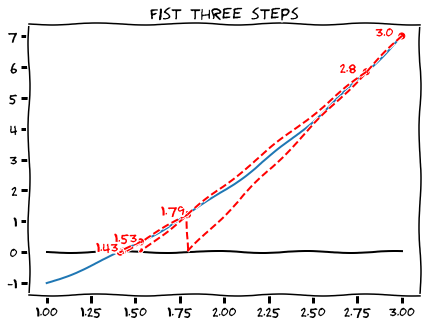
\includegraphics[width=0.6\linewidth]{images/secant.png}
\caption{Secant iterative method}
\end{figure}
\end{example}